\documentclass{classrep}
\usepackage[utf8]{inputenc}
\frenchspacing

\usepackage{graphicx}
\usepackage[usenames,dvipsnames]{color}
\usepackage[hidelinks]{hyperref}
\usepackage{lmodern}
\usepackage{graphicx}
\usepackage{placeins}
\usepackage{url}
\usepackage{amsmath, amssymb, mathtools}
\usepackage{listings}
\usepackage{fancyhdr, lastpage}

\pagestyle{fancyplain}
\fancyhf{}
\renewcommand{\headrulewidth}{0pt}
\cfoot{\thepage\ / \pageref*{LastPage}}

%--------------------------------------------------------------------------------------%

\studycycle{Informatyka, studia dzienne, I st.}
\coursesemester{VI}

\coursename{Komputerowe systemy rozpoznawania}
\courseyear{2019/2020}

\courseteacher{dr hab. inż. Adam Niewiadomski, prof. PŁ}
\coursegroup{poniedziałek, 12:00}

\author{
    \studentinfo{Jan Karwowski}{216793} \and
    \studentinfo{Kamil Kowalewski}{216806}
}

\title{Zadanie 1: Ekstrakcja cech, miary podobieństwa, klasyfikacja}

\begin{document}
    \maketitle
    \thispagestyle{fancyplain}

    \section{Cel} {
        Celem zadania jest stworzenie aplikacji do klasyfikacji zbiorów tekstów z wykorzystaniem
        klasyfikatora k-NN. W tym celu konieczne będzie przeprowadzenie ekstrakcji cech. Ostatecznie
        zbadany zostanie wpływ poszczególnych parametrów działania programu na jakość klasyfikacji.
    }
%--------------------------------------------------------------------------------------%
    \section{Wprowadzenie} {

        \subsection{k-NN} \label{knn} {
            Zadanie klasyfikacji, polegające na przydzielaniu obiektów do wcześniej zdefiniowanych grup
            można rozwiązać na różne sposoby. Powstało wiele algorytmów klasyfikujących, a spośród nich
            jednym z najprostszych co do zasady działania jest algorytm k-NN (\emph{ang. k-nearest neighbors}).
            Klasyfikator ten nie wymaga procesu uczenia, zbiór uczący jest jedynie przechowywany w pamięci
            programu a przetwarzany jest dopiero podczas właściwej klasyfikacji. Działanie tego algorytmu polega
            na znajdowaniu najbliższych (zgodnie z pewną miarą) obiektów ze zbioru uczącego dla każdego elementu
            ze zbioru testowego. Następnie klasa przetwarzanego obiektu zostaje rozpoznana jako najczęstsza spośród
            znalezionych wcześniej "sąsiadów". Algorytm można więc przedstawić w następujących krokach:
            \begin{enumerate}
                \item Weź jeden element ze zbioru testowego
                \item Znajdź $k$ najbliższych elementów ze zbioru uczącego
                \item Wybierz klasę najczęściej występującą pośród znalezionych elementów
                \item Wybrana klasa jest klasą rozpoznawanego elementu ze zbioru testowego
            \end{enumerate}
        }

        \subsection{Miary i metryki} \label{miary_metryki} {
            Aby znaleźć "sąsiadów" musi istnieć pewien sposób określania podobieństwa lub bliskości
            między przetwarzanymi obiektami. Ponadto zazwyczaj (w przypadku rzeczywistych obiektów - tekstów,
            obrazów, dźwięków) klasę obiektu można określić już na podstawie pewnego podzbioru wszystkich cech
            obiektu, czyli na podstawie pewnego \emph{obrazu obiektu}. Warto zwrócić uwagę, że takie podejście,
            polegające na braniu pod uwagę jedynie części cech opisujących obiekt, jest bardzo korzystne ze
            względu na wydajność działania programu. Aby dokonać klasyfikacji tekstów będzie więc trzeba wyekstrahować
            z nich pewne cechy i tak każdy tekst zostanie zamieniony na pewien N-wymiarowy wektor zawierający liczby lub
            słowa - cecha tekstu może być wynikiem pewnych operacji matematycznych lub po prostu pewnym fragmentem tekstu.
            Dopiero te wektory będą przetwarzane przez klasyfikator k-NN, a podobieństwo/odległość między nimi będzie
            określona za pomocą wybranej miary.

            Istnieje wiele metryk pozwalających obliczyć odległość między wektorami liczbowymi. Wynikiem ekstrakcji
            cech nie są jednak wektory zawierające wyłącznie liczby. Niektóre cechy jako swoje wartości przyjmują
            pojedyncze słowo. Aby obliczyć podobieństwo wektorów cech trzeba je najpierw zamienić na wektory liczbowe.
            Aby to zrobić musi istnieć pewna miara, pozwalająca określić, jak podobne są do siebie ciągi znaków. Podczas
            realizacji zadania zostały zaimplementowane dwie takie miary.

            \subsubsection{TFM - term frequency matrix} \label{tfm} {
                Zgodnie z definicją metoda ta pozwala określić podobieństwo ciągów wyrazów. Brany jest pewien zbiór słów
                kluczowych (mających decydujące znaczenie dla skuteczności metody) i w każdym dokumencie/tekście obliczana
                jest liczba wystąpień każdego słowa kluczowego - powstają w ten sposób wektory liczbowe. Następnie
                podobieństwo wektorów można obliczyć wykorzystując wybraną metrykę.

                W naszym przypadku potrzebujemy porównywać jedynie pojedyncze słowa. Zbiorem słów kluczowych stanie się
                więc jedno z dwóch porównywanych słów a wynik porównania tych ciągów znaków wyrażony będzie wzorem:
                \begin{equation}
                    sim(s_1, s_2) = \left\{ \begin{array}{ll}
                                                0 & \textrm{dla $s_1 \ne s_2$}\\
                                                1 & \textrm{dla $s_1 = s_2$}
                    \end{array}\right.
                \end{equation}
                gdzie $s_1$ i $s_2$ oznaczają łańcuchy znaków.
            }

            \subsubsection{Metoda n-gramów} \label{ngram} {
                Metoda polega na na określaniu podobieństwa łańcuchów tekstowych $s_1$, $s_2$
                na podstawie liczby n-gramów czyli wspólnych podciągów
                \begin{equation}
                    sim_n(s_1, s_2)=\frac{1}{N-n+1}\sum_{i=1}^{N-n+1} h(i)
                \end{equation}
                gdzie:\\
                $h(i)=1$ gdy n-elementowy podciąg zaczynający się od i-tej pozycji w $s_1$,
                występuje przynajmniej raz w $s_2$\\
                $N-n+1$ - liczba możliwych n-elementowych podciągów w $s_1$ \\

                W przypadku naszego programu pojedynczym n-gramem jest pojedyncza litera. Zastosowana
                została jedynie metoda trigramów, czyli metoda n-gramów dla ustalonego $n = 3$.
            }

            \subsubsection{Konwersja wektora cech na wektor liczbowy} {
                Wykorzystując opisane miary możemy pewną liczbą wyrazić podobieństwo dwóch łańcuchów znaków.
                Istnieje więc teraz możliwość, aby zamienić wektory cech, zawierające liczby lub słowa, na wektory
                zawierające jedynie liczby. Konwersja ta będzie przebiegała dopiero na etapie porównywania
                dwóch wybranych wektorów cech, w trakcie pracy algorytmu kNN. Konwersja pary wektorów cech $A$, $B$
                na wektory liczbowe $X$, $Y$ przebiega według następującego algorytmu:
                \begin{enumerate}
                    \item Znaleźć element $s_1$ wektora $A$, który zawiera ciąg znaków.
                    \item Obliczyć odległość $d = 1 - sim(s_1, s_2)$, gdzie $s_2$ jest równoległym
                    elementem w wektorze $B$. Wykorzystać wybraną miarę podobieństwa tekstów.
                    \item Do wektora $A$ wstawić w miejsce tekstu $s_1$ wartość $0$
                    \item Do wektora $B$ wstawić w miejsce tekstu $s_2$ wyliczoną wartość $d$
                    \item Powtarzać operację dopóki wektor $A$ zawiera elementy tekstowe
                \end{enumerate}
            }

            \subsubsection{Metryki} \label{metryka}{
                W opracowywanej aplikacji zostały wykorzystane trzy różne metryki,
                pozwalające określić jak bardzo bliskie siebie są N-wymiarowe wektory liczb rzeczywistych.
                \begin{itemize}
                    \item Metryka euklidesowa
                    $$
                    \rho_E(X,Y)= \sqrt{\sum^N_{i=1} (x_i-y_i)^2}
                    $$
                    \item Metryka uliczna (zwana także miejską lub taksówkową)
                    $$
                    \rho_C(X,Y)=\sum^N_{i=1}|x_i-y_i|
                    $$
                    \item Metryka Czebyszewa
                    $$
                    \rho_{\infty}(X,Y)= \max_{i=1,...,N} |x_{i} - y_{i}|
                    $$
                \end{itemize}
            }
        }

        \subsection{Ekstrakcja cech} {
            Aby zamienić teksty na łatwe w przetwarzaniu i zrozumiałe dla komputera wektory liczb rzeczywistych
            należy dokonać wspomnianej wcześniej ekstrakcji cech. Większość z nich, będzie opierać się o pewną
            globalną listę słów kluczowych, czyli słów mających największe znaczenie, niosących najwięcej informacji,
            spośród wszystkich słów tworzących badany zbiór tekstów.

            \subsubsection{Szukanie słów kluczowych} \label{keywords}{
                Zostały zastosowane dwie metody znajdowania słów kluczowych. Każda z nich pozwala wyznaczyć wartość
                pewnego parametru dla każdego słowa. Następnie na słowa kluczowe wybierane są te, dla których wartość
                ustalonego parametru jest największa.

                \paragraph{Term frequency - inverse document frequency (tf-idf)} {
                    Metoda ta pozwala określić jak ważne jest wybrane słowo dla danego dokumentu z uwzględniem faktu
                    czy występuje ono także w innych dokumentach w całym zbiorze. W ten sposób na słowa kluczowe wybrane zostaną
                    te, które występują często w skali jednego dokumentu ale rzadko w skali wszystkich dokumentów - słowa
                    charakteryzujące pojedynczy dokument. Aby obliczyć wartość parametru \emph{tf-idf} dla słowa $w$ w dokumencie
                    $d$, należy obliczyć kolejno wartości:
                    \begin{enumerate}
                        \item term frequency
                        \begin{equation}
                            tf_{w,d} = \frac{n_{w,d}}{N_{d}}
                        \end{equation}
                        gdzie $n_{w,d}$ - liczba wystąpień słowa $w$ w dokumencie $d$, $N_d$ - liczba wszystkich słów w dokumencie $d$
                        \item inverse document frequency
                        \begin{equation}
                            itf_{w} = \log\frac{|D|}{|\{d: w \in d\}|}
                        \end{equation}
                        gdzie $|{d: w \in d}|$ - liczba dokumentów zawierających przynajmniej jedno wystąpienie słowa $w$,
                        $|D|$ - liczba wszystkich dokumentów
                        \item \emph{tf-idf}
                        \begin{equation}
                            "tf-idf"_{w,d} = tf_{w,d} \cdot idf_{w}
                        \end{equation}
                    \end{enumerate}
                }


                \paragraph{Term frequency in class - inverse term frequency in other classes
                (tfc-itfoc)} {
                    Metoda ta pozwala określić jak ważne jest dane słowo dla pewnej klasy dokumentów. Jest to metoda autorska i bazuje
                    na przedstawionej wcześniej metodzie \emph{tf-idf}. W tym przypadku liczba wystąpień słowa $w$ jest określona dla całej
                    klasy (ile razy słowo wystąpiło we wszystkich dokumentach z tej klasy). Liczba dokumentów zawierających dane słowo
                    (document frequency) została zastąpiona liczbą wystąpień tego słowa we wszystkich pozostałych klasach. W ten sposób
                    na słowa kluczowe wybrane zostaną te, które występują często w pojedynczej klasie, ale w pozostałych występują rzadko.
                    Dla słowa $w$ z klasy $c$ należy obliczyć następujące parametry:
                    \begin{enumerate}
                        \item term frequency in class
                        \begin{equation}
                            tfc_{w,c} = \frac{n_{w,c}}{N_{c}}
                        \end{equation}
                        gdzie $n_{w,c}$ - liczba wystąpień słowa $w$ w dokumentach z klasy $c$, $N_c$ - liczba wszystkich słów w dokumentach klasy $c$
                        \item inverse term frequency in other classes
                        \begin{equation}
                            itfoc_{w,c} = \log\frac{1}{\left \{  \sum_{i=1 \land i \ne c}^{C} tfc_{w,i}\right \}}
                        \end{equation}
                        gdzie $tfc_{w,i}$ - liczba wystąpień słowa $w$ w klasie $i$, $C$ - wszystkie możliwe klasy dokumentów
                        \item \emph{tfc-itfoc}
                        \begin{equation}
                            "tfc-itfoc"_{w,c} = tfc_{w,c} \cdot itfoc_{w,c}
                        \end{equation}
                    \end{enumerate}
                }
            }

            \subsubsection{Cechy} {
                Z uwzględnieniem istnienia dwóch zbiorów $x$ słów kluczowych, które zostały wyznaczone opisanymi powyżej metodami
                ze zbioru wszystkich słów stanowiących przetwarzany zbiór tekstów (przed podziałem na zbiór uczący i testowy),
                wyekstrahowane zostały następujące cechy tekstów:
                \begin{enumerate}
                    \item Długość dokumentu - cecha ta oznacza liczbę słów danego dokumentu, pozwala zwiększyć dokładność
                    klasyfikacji obiektów przy założeniu, że dokumenty danej klasy średnio mają inną długość niż dokumenty klas pozostałych.
                    (Np. dokumenty klasy "usa" mogą być średnio o połowę dłuższe niż dokumenty klasy "uk")
                    \begin{equation}
                        len = N_{d}
                    \end{equation}
                    gdzie $N_{d}$ liczba słów w tekście $d$

                    \item Najczęstsze słowo we fragmencie dokumentu - wartością ekstrakcji tej cechy jest pojedyncze słowo, mające największą liczbę
                    wystąpień w wybranym fragmencie dokumentu.

                    \item Liczba wystąpień słów kluczowych we fragmencie dokumentu - cecha ta oznacza bezwzględną liczbę wystąpień słów ze zbioru słów kluczowych
                    w pewnym fragmencie (np. pierwszej połowie) dokumentu $d$. Cecha ta zwiększa dokładność klasyfikacji jeżeli niektóre klasy dokumentów
                    posiadają więcej wystąpień słów kluczowych niż inne. (Np. słowa kluczowe wykorzystane w dokumentach klasy "usa" powtarzają się częściej
                    niż w "uk"). Cecha ma także znaczenie jeżeli wykorzystany zbiór słów kluczowych będzie miał różne proporcje liczby słów charakterystycznych
                    dla poszczególnych klas.
                    \begin{equation}
                        k = |{w: w \in K \land w \in d_{part}}|
                    \end{equation}
                    gdzie $K$ - zbiór słów kluczowych, $d_{part}$ - zbiór słów stanowiących wybrany fragment dokumentu $d$ (uwzględniamy powtórzenia słowa!)

                    \item Względna liczba wystąpień słów kluczowych we fragmencie dokumentu - cecha ta oznacza stosunek liczby wystąpień słów ze zbioru słów kluczowych
                    w pewny fragmencie dokumentu $d$ do długości tego dokumentu. Znaczenie tej cechy jest podobne jak cechy poprzedniej. W tym przypadku
                    jednak, w połączeniu z cechą poprzednią, da się określić podobieństwo dokumentów o różnej długości, ale zbliżonym zagęszczeniu i
                    rozmieszczeniu słów kluczowych.
                    \begin{equation}
                        rk = \frac{|{w: w \in K \land w \in d_{part}}|}{|d_{part}|}
                    \end{equation}
                    gdzie $K$ - zbiór słów kluczowych, $d_{part}$ - zbiór słów stanowiących wybrany fragment dokumentu $d$ (uwzględniamy powtórzenia słowa!)

                    \item Liczba słów kluczowych we fragmencie dokumentu - cecha ta oznacza liczbę różnych słów kluczowych (bez uwzględnienia powtórzeń), które
                    pojawiają się we fragmencie dokumentu. Cecha ta pozwala rozróżnić od siebie dokumenty w przypadku, gdy któreś charakteryzują się różnorodnością
                    słów kluczowych a inne nie. (Np. dokumenty z klasy "usa" mogą mieć średnio 3 różne słowa kluczowe na dokument a z klasy "uk" 5 różnych słów
                    kluczowych).
                    \begin{equation}
                        uk = |{w: w \in K \land w \in d_{part}}|
                    \end{equation}
                    gdzie $K$ - zbiór słów kluczowych, $d_{part}$ - zbiór słów stanowiących wybrany fragment dokumentu $d$

                    \item najczęstsze słowo kluczowe we fragmencie dokumentu - ta cecha oznacza pojedyncze słowo spośród zbioru słów kluczowych, które najwięcej
                    razy wystapiło we fragmencie dokumentu
                \end{enumerate}

                Pierwsza cecha została dla danego dokumentu obliczona jeden raz, druga dwa razy - dla pierwszej i drugiej połowy, wszystkie pozostałe zostały
                obliczone osobno dla pierwszej i drugiej połowy dokumentu, a także dla dwóch różnych zbiorów słów kluczowych - po cztery razy. W ten sposób
                powstało $1 + 1 \cdot 2 + 4 \cdot 4 = 19$ różnych cech podlegających ekstrakcji.
            }
        }

        \subsection{Miary jakości} \label{jakosc} {
            Aby ocenić jakość klasyfikacji wykorzystane zostały trzy miary
            jakości (~\cite{quality}). Pierwsza dotyczy całego procesu
            klasyfikacji. Dwie pozostałe odnoszą się do jakości klasyfikacji
            danej klasy dokumentów.
            \begin{description}
                \item[accuracy] jest to miara oznaczająca dokładność całej klasyfikacji
                \begin{equation}
                    \textrm{accuracy} = \frac{\textrm{liczba poprawnie zaklasyfikowanych dokumentów}}{\textrm{liczba wszystkich klasyfikowanych dokumentów}}
                \end{equation}
                \item[recall] oznacza odsetek poprawnie zaklasyfikowanych dla danej klasy
                \begin{equation}
                    \textrm{recall} = \frac{\textrm{liczba poprawnie zaklasyfikowanych do klasy X}}{\textrm{liczba dokumentów klasy X}}
                \end{equation}
                \item[precision] oznacza precyzję klasyfikacji elementów danej klasy
                \begin{equation}
                    \textrm{precision} = \frac{\textrm{liczba poprawnie zaklasyfikowanych do klasy X}}{\textrm{liczba wszystkich zaklasyfikowanych do klasy X}}
                \end{equation}
            \end{description}
        }
    }
%--------------------------------------------------------------------------------------%
    \section{Opis implementacji} {
        Program został przygotowany w języku Java, w wersji JDK 1.8. Do kontrolowania zależnościami
        projektu został użyty Apache Maven. Pliku pobrane ze wskazanego w instrukcji źródła~\cite{data}
        zostały umieszczone w folderze resources aby zapewnić dogodne miejsce do ich przechowywania.
        W celu zachowania czytelności i możliwości rozbudowy, klasy projektu zostały podzielone na
        pakiety. Poniżej został przedstaiony skrócony opis poszczególnych pakietów.

        \begin{figure}[!htbp]
            \centering
            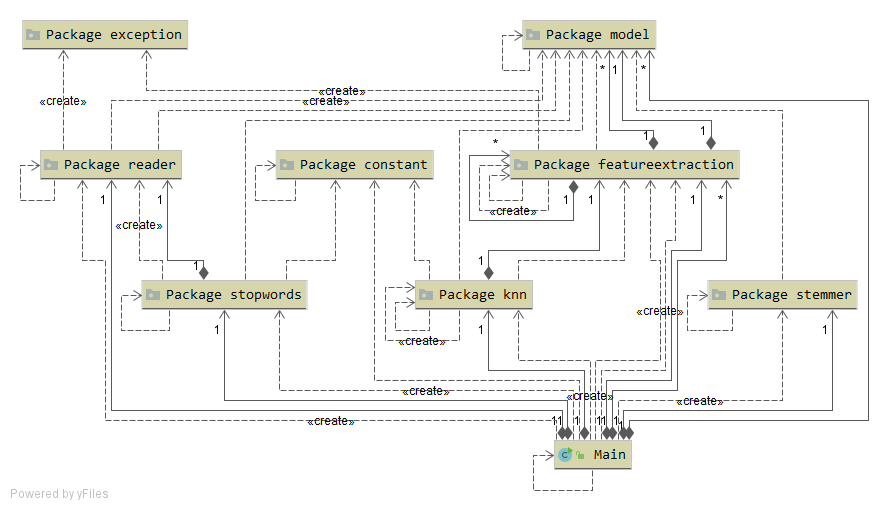
\includegraphics[width=\textwidth]{img/uml/wholeapp.png}
            \caption{Diagram UML całego projektu}
        \end{figure}
        \FloatBarrier

        \begin{description}
            \item[Pakiet \emph{knn}] zawiera implementację algorytmu knn
            \item[Pakiet \emph{model}] zawiera klasę modelu reprezentującą pojedyńczy artykuł ze zbioru danych,
                które są pobiera z plików, których źródłem jest ~\cite{data}.
            \item[Pakiet \emph{featureextraction}] zawiera klasy, które są odpowiedzialne za implemenetacje cech tekstów oraz
                modułu ich ekstrakcji. Posiada on też klasy odpowiedzialne za implementacje miar
                wykorzystywanych w programie. Aby zapewnić dogodne i szybkie dodawanie lub usuwanie
                cech został użyty wzorzec projektowy dekoratora.
            \item[Pakiet \emph{reader}] zawiera klasy odpowiedzialne za wczytywanie danych z plików w systemie operacyjnym. Do
                danych tych zaliczone są wszystkie dokumenty (~\cite{data}) oraz stoplista (uzyskana ze źródła~\cite{stoplist}).
                Wykorzystane zostały biblioteki JSoup~\cite{sgmlparser} oraz Gson~\cite{gson}.
            \item[Pakiet \emph{stemmer}] posiada klasę odpowiadająco za proces stemizacji słów. Jej implementacja została
                oparta o bibliotekę PorterStemmer~\cite{stemmer}.
            \item[Pakiet \emph{stopwords}] posiada klasę odpowiadająco za proces usuwania słów znajdujących się
                na stopliscie z artykułów.
            \item[Pakiety \emph{constant} i \emph{exception}] zawierają klasy wyjątków i zbiory stałych wykorzystywanych
                w programie.
            \item[Główna klasa programu \emph{Main}] Klasą posiada główną metodę programu, w której została w stosownej kolejności
                utworzone obiekty klas oraz zostały wywołane metody operujące na tych obiektach
                w celu wykorzystania zaimplementowanych mechanizmów w programie.
        \end{description}
    }
%--------------------------------------------------------------------------------------%

    \section{Materiały i metody} \label{materialy} {
%
        Aby użyć programu należy przekazać mu parametry uruchomieniowe. Pierwszym z nich
        jest procentowy podział zbioru na treningowy i testowy, gdzie podawaną wartością
        jest procent dla zbioru treningowego. Kolejnym parametrem jest liczba k najbliższych
        sąsiadów algorymtu knn opisanego w \ref{knn}. Trzecim argumentem jest liczba słów kluczowych.
        Do ostatnich dwóch argumentów należy metryka opisana w \ref{metryka} oraz miara do wyboru w
        dwóch wariantach opisanych w \ref{tfm} oraz \ref{ngram}. Po zakończeniu działanie
        programu na konsoli zostają wypisane statystyki działania programu w tym wartości
        Accuracy, Recall, Precision. Dane wyświetlane na konsoli zostają również zapisane
        automatycznie do pliku tekstowego, w którego nazwie znajdują się parametry wejściowe.\\

        Warto zaznaczyć, że przed poniższymi badaniami została wykonana analiza dla wielu
        kombinacji matryk, miar oraz liczby słów kluczowuch i została wybrana grupa
        dla, której wyniki były najlepsze.

        \subsection{Wpływ użytej wartość liczby k-najbliższych sąsiadów na jakość klasyfikacji} {
            W tej części został zbadany wpływ liczby k-najbliższych sąsiadów na skuteczość
            działania programu. Próba została przeprowadzona dla dziesięciu różnych wartość
            liczby k są to kolejno 1,3,5,7,9,11,13,15,17,19 i dla stałych wartości
            podziały zbioru równego 40\% dla części trenigowej i 60\% dla części testowej.
            Wybraną metryką była metryka euklidesowa natomiast miarą była term frequency matrix.
            Za każdym razem wykorzystano 10000 słów kluczowych.
        }

        \subsection{Wpływ podziału zbioru na treningowy i testowy na jakość klasyfikacji} {
            W tej części został zbadany wpływ podziału zbioru dla części trenigowej
            oraz dla części testowej. Wartościami dla jakiej był testowany wpływ są
            kolejno 30/70, 40/60, 50/50, 60/40, 70/30 gdzie pierwszą wartością jest procent
            zbioru treningowe natomiast drugą jest procent zbioru testowego. Stałymi parametrami
            była liczba k równa 9, liczba słów kluczowych równa 10000, wybrana metryka to
            metryka euklidesowa oraz miara term frequency matrix.
        }

        \subsection{Wpływ użytej metryki i miary na jakość klasyfikacji} {
            W tej części został zbadany wpływ wyboru metryki i miary. Ze względu na to, że
            do wyboru są trzy metryki oraz dwie miary daję to sześć kombinacji czyli sześciokrotne
            uruchomienie programu. Stałymi parametrami był podział zbioru równego 60\% dla
            części trenigowej i 40\% dla części testowej, wartość liczby k równej 3 oraz liczba
            słów kluczowych równa 10000.
        }

        \subsection{Wpływ użytych cech na jakość klasyfikacji} {
            Zostało wybranych 7 różnych pozbiorów zbioru wszystkich 19 cech. Dla każdego podzbioru
            przeprowadzony został jeden eksperyment. Wszystkie 7 eksperymentów zostało
            przeprowadzonych przy tych samych parametrach wejściowych programu.
            \begin{itemize}
                \item proporcja podziału - 60\%
                \item parametr \emph{k} - 3
                \item liczba słów kluczowych - 3000
                \item metryka euklidesowa
                \item miara podobieństwa tekstów TFM
            \end{itemize}
            Podzbiory zostały wybrane tak, aby zbadać wpływ poszczególnych cech na jakość
            klasyfikacji:
            \begin{enumerate}
                \item Wszystkie 19 cech
                \item Tylko cechy zależne od zbiorów słów kluczowych (cechy 3, 4, 5 i 6 dla dwóch
                    części dokumentu i dwóch zbiorów słów kluczowych)
                \item Tylko cechy niezależne od zbiorów słów kluczowych (cechy 1 i 2 dla dwóch
                    części dokumentów)
                \item Wszystkie cechy bez tych, wykorzystujących pierwszy (patrz \ref{keywords})
                    zestaw słów kluczowych (cechy 1, 2, 3, 4, 5, 6 dla dwóch części dokumentu, przy
                    czym 3, 4, 5, 6 tylko dla drugiego zbioru słów kluczowych)
                \item Wszystkie cechy bez tych, wykorzystujących drugi (patrz \ref{keywords}) zestaw
                    słów kluczowych (cechy 1, 2, 3, 4, 5, 6 dla dwóch części dokumentu, przy czym 3
                    ,4 ,5 ,6 tylko dla pierwszego zbioru słów kluczowych)
                \item Tylko cechy wykorzystujące pierwszą połowę każdego dokumentu (cechy 1, 2, 3,
                    4, 5, 6 dla pierwszej połowy dokumentu)
                \item Tylko cechy wykorzystujące drugą połowę każdego dokumentu (cechy 1, 2, 3, 4,
                    5, 6 dla drugiej połowy dokumentu)
            \end{enumerate}
        }
    }
%--------------------------------------------------------------------------------------%
    \section{Wyniki} {

        Poniżej zostały zaprezentowane wyniki przeprowadzony badań, które zostały
        opisane w sekcji \ref{materialy}.

        \subsection{Wpływ użytej wartość liczby k-najbliższych sąsiadów na jakość klasyfikacji} {

             \begin{table}[!htbp]
                \centering
                \begin{tabular}{|l|l|l|l|l|l|l|}
                    \hline
                    Numer                  & 1                  & 2             & 3             & 4             \\ \hline
                    Podział zbioru         & 60		            & 60		    & 60		    & 60		    \\ \hline
                    liczby K               & 1			        & 3			    & 5			    & 7			    \\ \hline
                    Liczba słów kluczowych & 10000		        & 10000		    & 10000		    & 10000		    \\ \hline
                    Metryka                & Euklidesowa	    & Euklidesowa 	& Euklidesowa	& Euklidesowa	\\ \hline
                    Miara                  & TFM		        & TFM		    & TFM		    & TFM		    \\ \hline
                    Accuracy {[}\%{]}      & 71,59		        & 74,01		    & 76,53		    & 77,52		    \\ \hline
                    Czas wykonania {[}s{]} & 94,00		        & 96,72		    & 109,09	    & 141,50	    \\ \hline
                    USA Recall             & 0,85		        & 0,90		    & 0,94		    & 0,96		    \\ \hline
                    USA Precision          & 0,84		        & 0,83		    & 0,82		    & 0,81		    \\ \hline
                    CANADA Recall          & 0,15		        & 0,05		    & 0,05		    & 0,01		    \\ \hline
                    CANADA Precision       & 0,18		        & 0,22		    & 0,22		    & 0,15		    \\ \hline
                    JAPAN Recall           & 0,27		        & 0,10		    & 0,12		    & 0,10		    \\ \hline
                    JAPAN Precision        & 0,29		        & 0,16		    & 0,23		    & 0,26		    \\ \hline
                    UK Recall              & 0,32		        & 0,26		    & 0,22		    & 0,17		    \\ \hline
                    UK Precision           & 0,29		        & 0,30		    & 0,32		    & 0,32		    \\ \hline
                    FRANCE Recall          & 0,11		        & 0,08		    & 0,03		    & 0,02		    \\ \hline
                    FRANCE Precision       & 0,10		        & 0,08		    & 0,07		    & 0,09		    \\ \hline
                    WEST-GERMANY Recall    & 0,19		        & 0,19		    & 0,11		    & 0,06		    \\ \hline
                    WEST-GERMANY Precision & 0,18		        & 0,16		    & 0,22		    & 0,19		    \\ \hline
                    \end{tabular}
                    \caption{Wartości wejściowe i wyjściowe programu przy badaniu wpływu liczby \emph{k} na jakość klasyfikacji} \label{table-k1}
                \end{table}
                \FloatBarrier

               \begin{table}[!htbp]
                \centering
                \begin{tabular}{|l|l|l|l|l|l|l|}
                    \hline
                    Numer                    & 5            & 6           & 7           \\ \hline
                    Podział zbioru           & 60			& 60		  & 60		    \\ \hline
                    liczby K                 & 9			& 11		  & 13		    \\ \hline
                    Liczba słów kluczowych   & 10000		& 10000		  & 10000		\\ \hline
                    Metryka                	 & Euklidesowa	& Euklidesowa & Euklidesowa	\\ \hline
                    Miara                    & TFM			& TFM		  & TFM		    \\ \hline
                    Accuracy {[}\%{]}        & 78,53		& 78,70		  & 79,06		\\ \hline
                    Czas wykonania {[}s{]}   & 118,36	    & 113,02	  & 123,56	    \\ \hline
                    USA Recall               & 0,97		    & 0,98		  & 0,99		\\ \hline
                    USA Precision            & 0,81		    & 0,81		  & 0,80		\\ \hline
                    CANADA Recall            & 0,02		    & 0,01		  & 0,01		\\ \hline
                    CANADA Precision         & 0,24		    & 0,29		  & 0,30		\\ \hline
                    JAPAN Recall             & 0,07		    & 0,07		  & 0,06		\\ \hline
                    JAPAN Precision          & 0,26		    & 0,31		  & 0,36		\\ \hline
                    UK Recall                & 0,15		    & 0,13		  & 0,12		\\ \hline
                    UK Precision             & 0,36		    & 0,34		  & 0,41		\\ \hline
                    FRANCE Recall            & 0,01		    & 0,00		  & 0,01		\\ \hline
                    FRANCE Precision         & 0,12		    & 0,00		  & 0,50		\\ \hline
                    WEST-GERMANY Recall      & 0,07		    & 0,07		  & 0,02		\\ \hline
                    WEST-GERMANY Precision   & 0,41		    & 0,56		  & 0,33		\\ \hline
                    \end{tabular}
                    \caption{Wartości wejściowe i wyjściowe programu przy badaniu wpływu liczby \emph{k} na jakość klasyfikacji (cd.)} \label{table-k2}
                \end{table}
                \FloatBarrier

                \begin{table}[!htbp]
                \centering
                \begin{tabular}{|l|l|l|l|l|l|l|}
                    \hline
                    Numer                   & 8           & 9               & 10               \\ \hline
                    Podział zbioru          & 60		  & 60		        & 60		      \\ \hline
                    liczby K                & 15		  & 17		        & 19		      \\ \hline
                    Liczba słów kluczowych  & 10000		  & 10000		    & 10000		      \\ \hline
                    Metryka                	& Euklidesowa & Euklidesowa	    & Euklidesowa	  \\ \hline
                    Miara                   & TFM		  & TFM		        & TFM		      \\ \hline
                    Accuracy {[}\%{]}       & 78,90		  & 78,84		    & 78,86		      \\ \hline
                    Czas wykonania {[}s{]}  & 126,52	  & 136,51	        & 120,35	      \\ \hline
                    USA Recall              & 0,99		  & 0,99		    & 0,99		      \\ \hline
                    USA Precision           & 0,80		  & 0,80		    & 0,80		      \\ \hline
                    CANADA Recall           & 0,00		  & 0,00		    & 0,00		      \\ \hline
                    CANADA Precision        & 0,33		  & 1,00		    & 1,00		      \\ \hline
                    JAPAN Recall            & 0,05		  & 0,03		    & 0,01		      \\ \hline
                    JAPAN Precision         & 0,33		  & 0,32		    & 0,19		      \\ \hline
                    UK Recall               & 0,11		  & 0,10		    & 0,10		      \\ \hline
                    UK Precision            & 0,39		  & 0,38		    & 0,40		      \\ \hline
                    FRANCE Recall           & 0,00		  & 0,00		    & 0,00		      \\ \hline
                    FRANCE Precision        & 0,00		  & 0,00		    & 0,00		      \\ \hline
                    WEST-GERMANY Recall     & 0,02		  & 0,02		    & 0,01		      \\ \hline
                    WEST-GERMANY Precision  & 0,38		  & 0,40		    & 0,50		      \\ \hline
                    \end{tabular}
                    \caption{Wartości wejściowe i wyjściowe programu przy badaniu wpływu liczby \emph{k} na jakość klasyfikacji (cd.)} \label{table-k3}
                \end{table}
                \FloatBarrier

            \begin{figure}[!htbp]
                \centering
                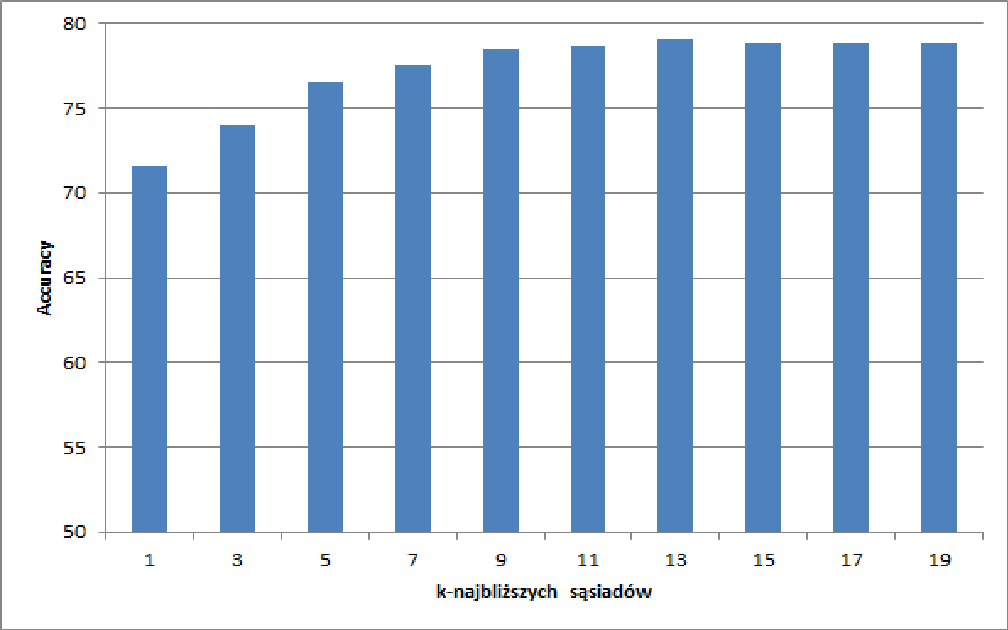
\includegraphics[width=\textwidth]{img/chart/accuracy_k.png}
                \caption{Zależność \emph{accuracy} od liczby \emph{k} przy stałych pozostałych parametrach} \label{chart-k}
            \end{figure}
            \FloatBarrier
        }

        \subsection{Wpływ podziału zbioru na treningowy i testowy na jakość klasyfikacji} {

            \begin{table}[!htbp]
                \centering
                \begin{tabular}{|l|l|l|l|l|l|l|}
                    \hline
                    Numer                  & 1              & 2             & 3                \\ \hline
                    Podział zbioru         & 30		        & 40		    & 50		       \\ \hline
                    liczby K               & 9			    & 9			    & 9			       \\ \hline
                    Liczba słów kluczowych & 10000		    & 10000		    & 10000		       \\ \hline
                    Metryka                & Euklidesowa	& Euklidesowa	& Euklidesowa	   \\ \hline
                    Miara                  & TFM		    & TFM		    & TFM		       \\ \hline
                    Accuracy {[}\%{]}      & 78,92		    & 78,98		    & 78,57		       \\ \hline
                    Czas wykonania {[}s{]} & 104,95	        & 114,53	    & 139,26	       \\ \hline
                    USA Recall             & 0,98		    & 0,98		    & 0,97		       \\ \hline
                    USA Precision          & 0,81		    & 0,81		    & 0,81		       \\ \hline
                    CANADA Recall          & 0,01		    & 0,02		    & 0,02		       \\ \hline
                    CANADA Precision       & 0,18		    & 0,47		    & 0,28		       \\ \hline
                    JAPAN Recall           & 0,03		    & 0,06		    & 0,06		       \\ \hline
                    JAPAN Precision        & 0,21		    & 0,36		    & 0,25		       \\ \hline
                    UK Recall              & 0,17		    & 0,17		    & 0,15		       \\ \hline
                    UK Precision           & 0,41		    & 0,35		    & 0,36		       \\ \hline
                    FRANCE Recall          & 0,01		    & 0,01		    & 0,01		       \\ \hline
                    FRANCE Precision       & 0,08		    & 0,07		    & 0,05		       \\ \hline
                    WEST-GERMANY Recall    & 0,05		    & 0,03		    & 0,06		       \\ \hline
                    WEST-GERMANY Precision & 0,28		    & 0,32		    & 0,26		       \\ \hline
                    \end{tabular}
                    \caption{Wartości wejściowe i wyjściowe programu przy badaniu wpływu proporcji podziału na zbiór uczący i testowy na jakość klasyfikacji} \label{table-podzial1}
                \end{table}
                \FloatBarrier

            \begin{table}[!htbp]
                \centering
                \begin{tabular}{|l|l|l|l|l|l|l|}
                    \hline
                    Numer                    & 4                & 5        \\ \hline
                    Podział zbioru           & 60		        & 70		\\ \hline
                    liczby K                 & 9			    & 9		    \\ \hline
                    Liczba słów kluczowych   & 10000		    & 10000	    \\ \hline
                    Metryka                  & Euklidesowa	    & Euklidesowa \\ \hline
                    Miara                    & TFM		        & TFM		\\ \hline
                    Accuracy {[}\%{]}        & 78,53		    & 79,05	    \\ \hline
                    Czas wykonania {[}s{]}   & 132,41	        & 123,82	\\ \hline
                    USA Recall               & 0,97		        & 0,98		\\ \hline
                    USA Precision            & 0,81		        & 0,81		\\ \hline
                    CANADA Recall            & 0,02		        & 0,03		\\ \hline
                    CANADA Precision         & 0,24		        & 0,44		\\ \hline
                    JAPAN Recall             & 0,07		        & 0,06		\\ \hline
                    JAPAN Precision          & 0,26		        & 0,29		\\ \hline
                    UK Recall                & 0,15		        & 0,18		\\ \hline
                    UK Precision             & 0,36		        & 0,43		\\ \hline
                    FRANCE Recall            & 0,01		        & 0,01		\\ \hline
                    FRANCE Precision         & 0,12		        & 0,17		\\ \hline
                    WEST-GERMANY Recall      & 0,07		        & 0,06		\\ \hline
                    WEST-GERMANY Precision   & 0,41		        & 0,29		\\ \hline
                    \end{tabular}
                    \caption{Wartości wejściowe i wyjściowe programu przy badaniu wpływu proporcji podziału na zbiór uczący i testowy na jakość klasyfikacji} \label{table-podzial2}
                \end{table}
                \FloatBarrier

            \begin{figure}[!htbp]
                \centering
                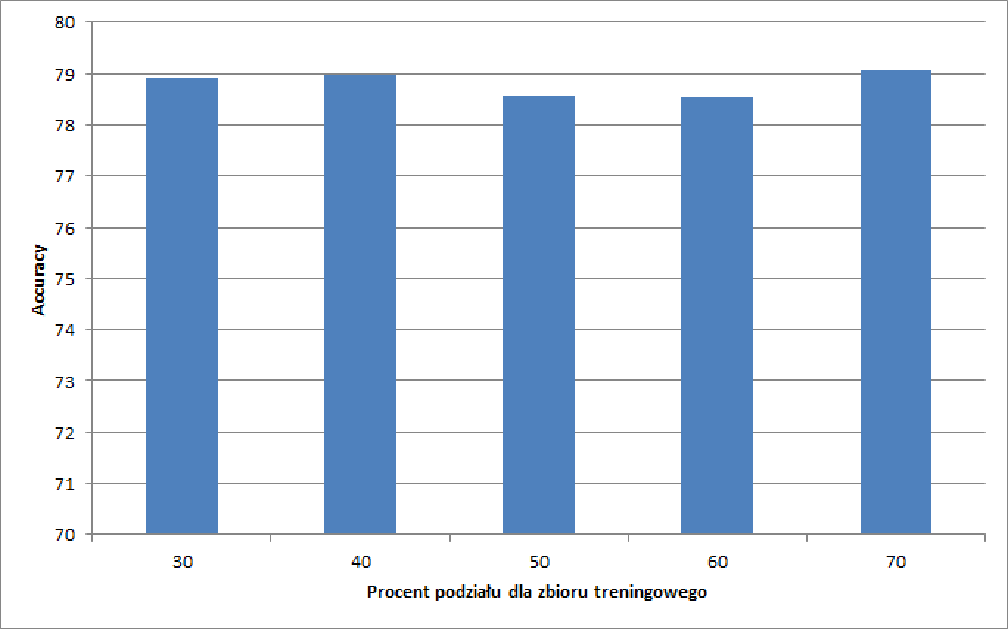
\includegraphics[width=\textwidth]{img/chart/accuracy_training_set.png}
                \caption{Zależność \emph{accuracy} od proporcji podziału danych na zbiory uczący i testowy przy stałych pozostałych parametrach} \label{chart-podzial}
            \end{figure}
            \FloatBarrier
        }

        \subsection{Wpływ użytej metryki i miary na jakość klasyfikacji} {
            \begin{table}[!htbp]
                \centering
                \begin{tabular}{|l|l|l|l|l|l|l|}
                    \hline
                    Numer                   & 1                 & 2           & 3            \\ \hline
                    Podział zbioru          & 60		        & 60		  & 60		     \\ \hline
                    liczby K                & 3			        & 3			  & 3			 \\ \hline
                    Liczba słów kluczowych  & 10000		        & 10000		  & 10000		 \\ \hline
                    Metryka                 & Euklidesowa	    & MANHATTAN	  & CHEBYSHEV	 \\ \hline
                    Miara                   & TFM		        & TFM		  & TFM		     \\ \hline
                    Accuracy {[}\%{]}       & 74,01		        & 74,17		  & 79,02		 \\ \hline
                    Czas wykonania {[}s{]}  & 99,30		        & 100,45	  & 100,11	     \\ \hline
                    USA Recall              & 0,90		        & 0,90		  & 1,00		 \\ \hline
                    USA Precision           & 0,83		        & 0,83		  & 0,79		 \\ \hline
                    CANADA Recall           & 0,05		        & 0,06		  & 0,00		 \\ \hline
                    CANADA Precision        & 0,22		        & 0,25		  & NaN			 \\ \hline
                    JAPAN Recall            & 0,10		        & 0,11		  & 0,00		 \\ \hline
                    JAPAN Precision         & 0,16		        & 0,20		  & NaN			 \\ \hline
                    UK Recall               & 0,26		        & 0,26		  & 0,03		 \\ \hline
                    UK Precision            & 0,30		        & 0,29		  & 0,67		 \\ \hline
                    FRANCE Recall           & 0,08		        & 0,12		  & 0,00		 \\ \hline
                    FRANCE Precision        & 0,08		        & 0,10		  & 0,00		 \\ \hline
                    WEST-GERMANY Recall     & 0,19		        & 0,19		  & 0,02		 \\ \hline
                    WEST-GERMANY Precision  & 0,16		        & 0,15		  & 1,00		 \\ \hline
                \end{tabular}
                \caption{Wartości wejściowe i wyjściowe programu przy badaniu wpływu użytej metryki i miary na jakość klasyfikacji}
            \end{table}
                \FloatBarrier

            \begin{table}[!htbp]
                \centering
                    \begin{tabular}{|l|l|l|l|l|l|l|}
                    \hline
                        Numer                  & 4                  & 5          & 6                \\ \hline
                        Podział zbioru         & 60		            & 60		 & 60		        \\ \hline
                        liczby K               & 3			        & 3			 & 3			 	\\ \hline
                        Liczba słów kluczowych & 10000		        & 10000		 & 10000		 	\\ \hline
                        Metryka                & Euklidesowa	    & MANHATTAN	 & CHEBYSHEV	 	\\ \hline
                        Miara                  & TRIGRAM	        & TRIGRAM	 & TRIGRAM	        \\ \hline
                        Accuracy {[}\%{]}      & 78,64		        & 78,46		 & 78,90		     \\ \hline
                        Czas wykonania {[}s{]} & 174,59	            & 285,05	 & 272,33	        \\ \hline
                        USA Recall             & 1,00		        & 0,99		 & 1,00		        \\ \hline
                        USA Precision          & 0,79		        & 0,79		 & 0,79		        \\ \hline
                        CANADA Recall          & 0,01		        & 0,01		 & 0,00		        \\ \hline
                        CANADA Precision       & 0,67		        & 0,67		 & NaN			     \\ \hline
                        JAPAN Recall           & 0,00		        & 0,00		 & 0,00		        \\ \hline
                        JAPAN Precision        & 0,00		        & 0,00		 & NaN			     \\ \hline
                        UK Recall              & 0,01		        & 0,01		 & 0,00		        \\ \hline
                        UK Precision           & 0,30		        & 0,11		 & NaN			     \\ \hline
                        FRANCE Recall          & 0,00		        & 0,00		 & 0,00		        \\ \hline
                        FRANCE Precision       & NaN			    & 0,00		 & NaN			     \\ \hline
                        WEST-GERMANY Recall    & 0,02		        & 0,01		 & 0,00		        \\ \hline
                        WEST-GERMANY Precision & 0,09		        & 0,05		 & NaN			     \\ \hline
                    \end{tabular}
                \caption{Wartości wejściowe i wyjściowe programu przy badaniu wpływu użytej metryki i miary na jakość klasyfikacji (cd.)}
            \end{table}
            \FloatBarrier

            \begin{figure}[!htbp]
                \centering
                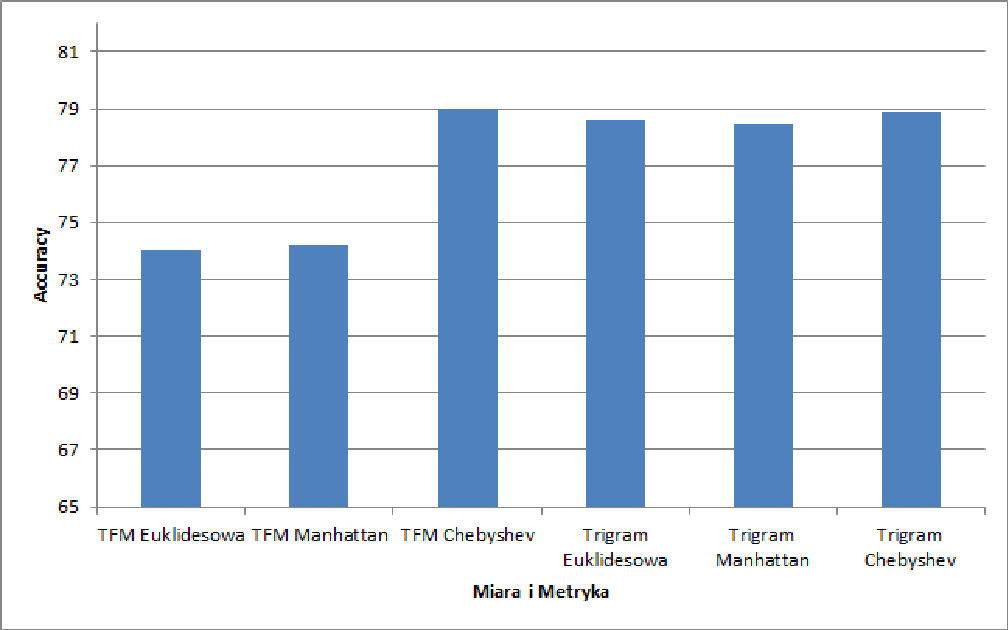
\includegraphics[width=\textwidth]{img/chart/accuracy_metric.png}
                \caption{Zależność \emph{accuracy} od użytej metryki i miary przy stałych pozostałych parametrach} \label{table-metric}
            \end{figure}
            \FloatBarrier
        }

        \subsection{Wpływ użytych cech na jakość klasyfikacji} {

            \begin{table}[!htbp]
                \centering
                \begin{tabular}{|l|l|l|l|l|l|l|}
                    \hline
                    Numer podzbioru cech   & 1     & 2     & 3     & 4     \\ \hline
                    Accuracy {[}\%{]}      & 74.30 & 73.19 & 73.47 & 74.39 \\ \hline
                    Czas wykonania {[}s{]} & 57.80 & 42.31 & 25.40 & 44.58 \\ \hline
                    USA Recall             & 0.89  & 0.90  & 0.89  & 0.90  \\ \hline
                    USA Precision          & 0.84  & 0.81  & 0.83  & 0.84  \\ \hline
                    CANADA Recall          & 0.04  & 0.02  & 0.04  & 0.04  \\ \hline
                    CANADA Precision       & 0.17  & 0.14  & 0.15  & 0.16  \\ \hline
                    JAPAN Recall           & 0.15  & 0.02  & 0.13  & 0.17  \\ \hline
                    JAPAN Precision        & 0.25  & 0.09  & 0.22  & 0.26  \\ \hline
                    UK Recall              & 0.25  & 0.11  & 0.23  & 0.26  \\ \hline
                    UK Precision           & 0.26  & 0.13  & 0.27  & 0.28  \\ \hline
                    FRANCE Recall          & 0.16  & 0.08  & 0.09  & 0.09  \\ \hline
                    FRANCE Precision       & 0.16  & 0.11  & 0.10  & 0.09  \\ \hline
                    WEST-GERMANY Recall    & 0.38  & 0.29  & 0.22  & 0.36  \\ \hline
                    WEST-GERMANY Precision & 0.26  & 0.26  & 0.15  & 0.25  \\ \hline
                \end{tabular}
                \caption{Wartości wejściowe i wyjściowe programu przy badaniu wpływu poszczególnych cech na jakość klasyfikacji} \label{table-features1}
            \end{table}
            \FloatBarrier

            \begin{table}[!htbp]
                \centering
                \begin{tabular}{|l|l|l|l|l|l|l|}
                    \hline
                    Numer podzbioru cech   & 5     & 6     & 7     \\ \hline
                    Accuracy {[}\%{]}      & 73.61 & 75.46 & 72.67 \\ \hline
                    Czas wykonania {[}s{]} & 44.85 & 26.89 & 37.36 \\ \hline
                    USA Recall             & 0.89  & 0.92  & 0.89  \\ \hline
                    USA Precision          & 0.83  & 0.82  & 0.82  \\ \hline
                    CANADA Recall          & 0.03  & 0.06  & 0.04  \\ \hline
                    CANADA Precision       & 0.15  & 0.14  & 0.20  \\ \hline
                    JAPAN Recall           & 0.13  & 0.07  & 0.08  \\ \hline
                    JAPAN Precision        & 0.21  & 0.37  & 0.15  \\ \hline
                    UK Recall              & 0.24  & 0.22  & 0.20  \\ \hline
                    UK Precision           & 0.27  & 0.29  & 0.20  \\ \hline
                    FRANCE Recall          & 0.12  & 0.04  & 0.06  \\ \hline
                    FRANCE Precision       & 0.12  & 0.12  & 0.07  \\ \hline
                    WEST-GERMANY Recall    & 0.20  & 0.16  & 0.24  \\ \hline
                    WEST-GERMANY Precision & 0.14  & 0.24  & 0.19  \\ \hline
                \end{tabular}
                \caption{Wartości wejściowe i wyjściowe programu przy badaniu wpływu poszczególnych cech na jakość klasyfikacji (cd.)} \label{table-features2}
            \end{table}
            \FloatBarrier
        }
    }
%--------------------------------------------------------------------------------------%
    \section{Dyskusja} {

        \subsection{Badanie wpływu parametru \emph{k} na jakość klasyfikacji} {
            Jak widzimy na wykresie \ref{chart-k} wartość \emph{accuracy} zmienia się wraz z ze
            zmianą parametru \emph{k}. Jednoznacznie można więc stwierdzić, że parametr ten ma wpływ
            na jakość klasyfikacji. Widać również, że jakość klasyfikacji (rozumiana jako
            \emph{accuracy}) zwiększa się wraz ze wzrostem liczby k, kiedy ten drugi parametr
            przyjmuje wartości w przedziale od 1 do 9. Następnie jakość klasyfikacji ulega
            stabilizacji. Opisane zależności wynikają bezpośrednio z wykresu \ref{chart-k}. Po
            przeanalizowaniu nie tylko wartości \emph{accuracy}, ale również wartości \emph{recall}
            oraz \emph{precision}, które to są wyliczane dla każdej klasy uwzględnionej w procesie
            klasyfikacji, okazuje się, że \emph{pierwsze wnioski są bardzo mylne}.

            W tabelach \ref{table-k1}, \ref{table-k2} i \ref{table-k3} przedstawione zostały
            szczegułowe wyniki działania programu podczas badania znaczenia parametru \emph{k}.
            Okazuje się, że dla każdej klasy, z wyłączeniem USA, wartość \emph{recall} maleje, wraz
            ze wzrostem wartości \emph{k}. W przypadku klasy USA, wartość ta rośnie. Oznacza to, że
            coraz więcej obiektów jest klasyfikowanych jako USA, co skutkuje bezpośrednio wzrostem
            wartości tej miary jakości klasyfikacji dla klasy USA, a zmniejszeniem tej wartości dla
            klas pozostałych.

            Wniosek ten uzupełnia przebieg zmian miary \emph{precision}, która oznacza ile spośród
            zaklasyfikowanych do danej klasy obiektów, zostało zaklasyfikowanych poprawnie. Wartość
            tej miary nie zachowuje się tak regularnie, jak wartość dwóch poprzednich. W niektórych
            przypadkach rośnie, w innych maleje, w jeszcze innych skacze w różnych kierunkach. W
            przypadku wszystkich klas poza klasą USA, wartość ta zachowuje się właściwie cały czas
            nieregularnie, jedynie warto zauważyć, że na sam koniec, może czasem osiągnąć wartość
            równą 1.  W przypadku klasy USA wartość ta konsekwentnie maleje. Sytuacja ta jest
            spowodowana faktem, że wraz ze wzrostem wartości parametru \emph{k}, liczba dokumentów
            klasyfikowanych jako USA drastycznie rośnie, aż w końcu prawie wszystkie (poza
            kilkunastoma) dokumenty są zaklasyfikowane jako USA. Wtedy też wartość miary
            \emph{precision} może zbliżyć się do 1, kiedy to wszystkie zaklasyfikowane do danej
            grupy dokumenty (bo jest ich tylko kilka) są zaklasyfikowane poprawnie. Taka ostatnia
            sytuacja ma miejsce, kiedy np. tylko jeden dokument zaklasyfikowano do UK i
            zaklasyfikowano go poprawnie. Wtedy to \emph{precision} osiąga wartość 1.

            Warto się zastanowić, dlaczego wraz ze wzrostem \emph{k} coraz więcej dokumentów
            jest klasyfikowanych jako USA. Wynika to z faktu, że klasa ta, jest znacznie liczniejsza
            od pozostałych. Liczba dokumentów faktycznie należących do grupy USA wynosi ok 80\%
            wszystkich dokumentów. Dlatego też właśnie ok 80\% wynosi ostatecznie i po
            ustabilizowaniu wartość \emph{accuracy}. Okazuje się więc, że \emph{accuracy} nie jest
            wcale najlepszą miarą jakości klasyfikacji, bo ostatecznie można stwierdzić, że wbrew
            temu co wyraża wartość tej miary, w tym konkretnym doświadczeniu, przy wybranych cechach
            do ekstrakcji i innych parametrach działania programu oraz w przypadku tego konretnego
            zbioru danych - \emph{jakość klasyfikacji maleje wraz ze wzrostem \emph{k}}. Dochodzi
            tu do sytuacji, kiedy jedna klasa dominuje pozostałe i przy zbyt dużej wartości
            parametru \emph{k} wszystkie dokumenty są "przyciągane" do tej jednej klasy.
        }

        \subsection{Badanie wpływu proporcji podziału na zbiory uczący i testowy na jakość klasyfikacji} \label{exper-test-set} {
            Na wykresie \ref{chart-podzial} widac zmiany wartości miary \emph{accuracy} przy różnym
            podziale na zbiór uczący i testowy. Można zauważyć, że nie mamy tu do czynienia z dużymi
            różnicami w jakości klasyfikacji, otrzymane liczby mieszczą się w przedziale między 78\%
            a 79\%. Są to więc różnice bardzo nieznaczne. Po przeanalizowaniu tabel
            \ref{table-podzial1} i \ref{table-podzial2} mozna stwierdzic, ze program zachowuje sie
            wlasciwie bardzo podobnie. Jak opisano w poprzednim rozdziale, wiekszosc dokumentow jest
            klasyfikowanych jako USA, co jest głównym powodem, dla którego oglądamy takie wartości
            miar jakości klasyfikacji, a nie inne. Można więc spróbować wysnuć dwa wnioski. Po
            pierwsze, że wraz ze wzrostem liczby elementów w zbiorze uczącym, wcale nie musi (na co
            by wskazywała intuicja) rosnąć dokładność klasyfikacji. Należy jednak zauważyć, że
            ponieważ zbiór jest pomieszany (dokumenty z danej klasy rozsiane są po całym zbiorze
            dokumentów), to różne wartości miar jakości klasyfikacji mogą wynikać z tego, że przy
            dołączaniu kolejnej części zbioru dokumentów do zbioru uczącego, może zmienić się
            proporcja liczności danych klas, w zbiorach uczących i testowych. Drugi wniosek,
            powiązany z pierwszym, jest więc taki, że po pewnej granicznej wartości (która nie
            zostałą tu zlokalizowana), zwiększenie zbioru uczącego może już nie zmieniać jakości
            klasyfikacji, co można zinterpretować jako, że klasyfikator nie może się już lepiej
            nauczyć.
        }

        \subsection{Badanie wpływu wybranej metryki i miary podobieństwa tekstów na jakość klasyfikacji} {
            Na wykresie \ref{table-metric} zostały przedstawione zmiany wartości miary \emph{accuracy}
            przy użyciu wszystkich sześciu kombinacji miar i metryk. Można zauważyć, że dla wszystkich
            kombinacji metryk i miar poza dwiema kombinacjami \emph{Euklides TFM} oraz \emph{Manhattan TFM}, różnica
            pomiędzy otrzymanymi wartościami \emph{accuracy} nie przekracza 1\% i tak jak w przypadku
            powyższego doświadczenia \ref{exper-test-set} wartość są z zakresu 78\% a 79\%. Stosunkowo
            duże różnice w porównianiu do reszty kombinacji można zauważyć dla kombinacji
            \emph{Euklides TFM} oraz \emph{Manhattan TFM} i wynoszą one około 5\%. W pierwszej chwili można uznać,
            że dla tych dwóch kombinacji został uzyskany gorszy wynik jednak jest to mylne gdyż
            inne klasy niż USA zostały o wiele lepiej zaklasyfikowane niż w pozostałych
            przypadkach gdzie praktycznie wszystkie inne klasy zostały określone jako klasa
            USA. Z tego przypadku płynie bardzo ciekawy wniosek, które jest prawdziwy dla tego
            zbioru danych zdominawanego przez klasę USA, że wysoką wartość parametru \emph{accuracy}
            nie musi oznaczać dobrej i wysokiej jakości klasyfikacji. Z uzyskanych wyników
            można też wnioskować, że dla miary Trigram wybór metryki w bardzo nieznaczny sposób
            wpływa na wyniki klasyfikacji natomiast dla miary TFM zauważalna jest wyraźna różnica.
            Jest to szczególnie widoczne porównująć metrykę Chebysheva do pozostałych użytych w eksperymencie.
        }

        \subsection{Badanie wpływu poszczególnych cech na jakość klasyfikacji} {
            Bardzo interesujące jest to, które spośród wymyślonych cech dokumentów mają kluczowe
            znaczenie w procesie klasyfikacji. Wyznaczonych zostało 7 podzbiorów cech i dla każdego
            takiego podzbioru przeprowadzono eksperyment. Tabele \ref{table-features1} oraz
            \ref{table-features2} prezentują wyniki tych eksperymentów. Po pierwsze można
            zauważyć, że wartość miary \emph{accuracy} zmienia się przy różnych cechach, co
            pozwala stwierdzić, że różne cechy mają różny wpływ na jakość klasyfikacji. Najwyższa
            wartość \emph{accuracy} widnieje przy podzbiorze 6. Można stąd wysnuć bardzo ważny
            wniosek. Okazuje się, że kluczowa dla określenia podobieństwa dokumentów jest ich
            pierwsza część. To co znajduje się w drugiej połowie nie tylko jest zbędne, przy
            ocenianiu, do której klasy dokument należy, ale także klasyfikację utrudnia. Potwierdza
            to fakt, że wartość \emph{accuracy} przy cechach zależnych od drugiej połowy każdego
            dokumentu jest najmniejsza, ze wszystkich otrzymanych w tej serii eksperymentów
            wartości.

            Różnica w jakości klasyfikacji pomiędzy podzbiorem 2 i 3 jest niewielka (zaledwie
            kilkadziesiąt setnych procenta). Można stąd wysnuć wniosek, że generalnie \emph{słowa
            kluczowe zostały wybrane bardzo nietrafnie}, ponieważ fakt, czy wykorzystujemy je w
            procesie klasyfikacji czy nie, nie wpływa zbytnio na jakość klasyfikacji. Po przyjrzeniu
            się innym miarom jakości \emph{precision} i \emph{recall} da się zauważyć, że w
            przypadku większości klas, wartości tych miar, zwiększają się wraz z zastosowaniem cech
            wykorzystujących słowa kluczowe. Ponieważ wartość \emph{accuracy} także (choć bardzo
            nieznacznie) zwiększa się w tym przypadku, można pokusić się o stwierdzenie, że
            wykorzystanie słów kluczowych poprawia jakość klasyfikacji. Jest to zachowanie zgodne z
            intuicją a oczekiwana poprawa jakości była znacznie większa, niż ta którą udało
            się tutaj osiągnąć.

            Otrzymane wyniki pozwalają porównać zastosowane algorytmy ekstrakcji słów kluczowych.
            Przy wykorzystaniu zbioru słów kluczowych otrzymanego w wyniku działania pierwszego
            algorytmu (tf-idf) otrzymaliśmy wartość \emph{accuracy} równą 73.61. Jest to prawie 1\%
            mniej niż w przypadku zastosowania algorytmu drugiego. Okazuje się więc, że autorska
            metoda ekstrakcji słów kluczowych, której zadaniem było wybrać słowa charakterystyczne
            dla danej klasy, w tym przypadku okazała się lepsza niż klasyczna, znana powszechnie
            metoda tf-idf.

            Na końcu, porównując eksperyment 1 z 6, warto zauważyć, że niektóre cechy mogą obniżać
            jakość klasyfikacji, a zrezygnowanie z nich tą jakość poprawi. W przeprowadzonych
            eksperymentach, wybrano jedynie kilka kombinacji spośród wszystkich wymyślonych cech,
            istnieje więc prawdopodobnie nieprzedstawiony tutaj podzbiór cech, dla którego jakość
            klasyfikacji była by jeszcze lepsza.
        }
    }
%--------------------------------------------------------------------------------------%
    \section{Wnioski} {
        \begin{itemize}
            \item Zbyt duża liczba obiektów w jednej klasie, w stosunku do liczb obiektów w klasach
                pozostałych bardzo utrudnia proces klasyfikacji metodą kNN
            \item Zwiększająca się wartość miary jakości \emph{accuracy} wcale nie oznacza, że
                klasyfikator rzeczywiście działa coraz lepiej
            \item Należy zawsze uwzględniać nie jedną, a kilka miar jakości klasyfikacji przy
                wysnuwaniu wniosków
            \item Zwiększenie wartości parametru \emph{k} w klasyfikatorze kNN może pogorszyć jakość
                klasyfikacji
            \item Proporcja podziału na zbiór uczący i testowy, w pewnym przedziale wartości nie
                musi mieć znaczącego wpływu na zmianę jakości klasyfikacji
            \item Niektóre cechy mogą obniżać jakoś klasyfikacji
            \item Podczas klasyfikacji tekstów, największe znaczenie ma to, co zostało napisane w
                początkowej części każdego z nich
            \item Podczas klasyfikacji tekstów, ważne jest w jaki sposób został pozyskany zbiór
                słów kluczowych
        \end{itemize}
    }
%--------------------------------------------------------------------------------------%
    \begin{thebibliography}{0}
        \bibitem{wyklad}{Niewiadomski, Adam. Materiały, przykłady i ćwiczenia do przedmiotu Komputerowe Systemy Rozpoznawania[online]. [dostęp 15.03.2020]. Dostępny w internecie: https://ftims.edu.p.lodz.pl/mod/folder/view.php?id=67970}
        \bibitem{commons}{Apache Commons Lang. Documentation[online]. [dostęp 15.03.2020]. Dostępny w internecie: https://commons.apache.org/proper/commons-lang/}
        \bibitem{sgmlparser}{JSoup. Documentation[online]. [dostęp 15.03.2020]. Dostępny w internecie: https://jsoup.org/cookbook/input/load-document-from-file}
        \bibitem{gson}{Google GSON. Documentation[online]. [dostęp 15.03.2020] .Dostępny w internecie: https://github.com/google/gson/blob/master/UserGuide.md}
        \bibitem{stemmer}{Apache OpenNLP. Documentation[online]. [dostęp 15.03.2020] .Dostępny w internecie: https://opennlp.apache.org/docs/1.7.2/apidocs/opennlp-tools/opennlp/\\tools/stemmer/PorterStemmer.html}
        \bibitem{stoplist}{CountWordsFree. English Stop Words[online]. [dostęp 15.03.2020]. Dostępny w internecie: https://countwordsfree.com/stopwords}
        \bibitem{agh}{Horzyk, Adrian. Metoda K Najbliższych sąsiadów[online]. [dostęp 15.03.2020]. Dostępny w internecie: http://home.agh.edu.pl/~horzyk/lectures/miw/MIW-KNN.pdf}
        \bibitem{data}{UCI. Reuters-21578 Text Categorization Collection Data Set[online]. [dostęp 15.03.2020]. Dostępny w internecie: https://archive.ics.uci.edu/ml/datasets/Reuters-21578+Text+Categorization+Collection}
        \bibitem{quality}{Tablica pomyłek[online]. [dostęp 15.04.2020] https://pl.wikipedia.org/wiki/Tablica\_pomyłek}
    \end{thebibliography}
\end{document}
